
\section{Software und Dienste}
Dieser Abschnitt behandelt die verwendete bzw. implementierte Software und die verwendeten Dienste für die Applikation \emph{RPISec}.

\subsection{\emph{Microservices}}
Dieser Abschnitt behandelt die auf dem \emph{Raspberry PI} gehosteten Services. Die Services wurden mit \emph{Spring Boot} als \emph{Microservices} implementiert, was möglich war, da Oracle eine ARM Implementierung der Java-JDK bereitstellt und die \emph{Microservices} schlank implementiert wurden, sodass die zur Verfügung stehenden Ressourcen ausreichen, um diese Services auf einen \emph{Raspberry PI} zu betreiben.
\newline
\newline
Es wurden die beiden \emph{Microservices Auth-Service} für die Benutzerverwaltung und OAuth2 Authentifizierung und \emph{App-Service} für die Interaktion mit der Sensorapplikation und der Interaktion mit dem \emph{Cloud} Dienst implementiert, wobei der \emph{Microservice Auth-service} im Zuge des Projekts für die Lehrveranstaltung \emph{Service Engineering} implementiert wurde. Es hätte auch ausgereicht die Benutzerverwaltung in den \emph{Microservice App-Service} zu verpacken, obwohl dann der \emph{Microservice} für zwei Aspekte verantwortlich gewesen wäre, was im Widerspruch zu einem \emph{Microservice} steht, der nur für einen Aspekt verantwortlich sein soll. 
\newline
\newline
Der \emph{Microservice App-Service} interagiert nicht direkt mit der Sensorik, sondern bindet die Sensorapplikation beschrieben in Abschnitt \ref{sec:sensor-application} ein und ist für dessen Lebenszyklus verantwortlich. Nachdem Start der Sensorapplikation wird ein \emph{Listener} registriert, der auf Statusänderungen des Bewegungssensor reagiert und diesen Sicherheitsverstoß wie in Abbildung \ref{fig:image-sequence-incident} behandelt.

\subsection{Datenbank}
Dieser Abschnitt behandelt die verwendete Datenbank für die \emph{Microservices}. Im Entwicklungsbetrieb auf einen Entwicklerrechner wird die Datenbank H2 und im produktiven Betrieb auf einen \emph{Raspberry PI} die Datenbank PostgreSQL verwendet. Die Datenbank PostgreSQL konnte am \emph{Raspberry PI} verwendet werden, da PostgreSQL die ARM Architektur unterstützt und sich auch mit geringen Ressourcenaufwand betreiben lässt.

\subsection{\emph{Cloud} Dienst}
Dieser Abschnitt behandelt den verwendeten \emph{Cloud} Dienst \emph{Firebase}. \emph{Firebase} ist ein \emph{Cloud} Dienst von \emph{Google}, der einen \emph{Messaging} Dienst sowie eine Onlinedatenbank (JSON-Datenbank) bereitstellt. Bis zu einer gewissen Anzahl von \emph{Requests} ist dieser Dienst kostenlos zu verwenden.  
\newline
\newline
Für \emph{Firebase} gibt es eine Java Implementierung das sogenannte \emph{firebase-admin-sdk}, das eine API zum Interagieren mit der JSON-Datenbank und eine API zum Erstellen von Authentifizierungstoken für die \emph{Client}-Authentifizierung auf \emph{Firebase} zur Verfügung stellt. In der Java Implementierung wird zurzeit keine API für die Interaktion mit dem \emph{Messaging} Dienst zur Verfügung gestellt, was aber kein Problem darstellt, da es sich hierbei um eine einfache Anfrage an eine \emph{REST-API} handelt, die mit Spring \emph{RestTemplate} realisiert wurde.
\newline
\newline
Für die Interaktion mit \emph{Firebase} über \emph{Android} wird ebenfalls eine Java Implementierung bereitgestellt. Diese Implementierung enthält auch eine \emph{API} für den \emph{MEssaging} Dienst von \emph{Firebase}.
\newline
\newline
Es sind zwar Implementierungen der \emph{API} mehrere Programmiersprachen verfügbar, jedoch wird eine vollständige \emph{API} nur für \emph{NodeJS} bereitgestellt.

\subsection{\emph{Docker}}
Dieser Abschnitt behandelt die Verwendung von \emph{Docker}, für das hosten der Services und Datenbanken für die Services. Dank dem \emph{Raspberry PI Image}, bereitgestellt von \emph{Hypriots}, sind bereits \emph{Docker} und \emph{Docker-Compose} \emph{(Orchestration)} vorinstalliert und müssen nicht separat geladen und für die Zielarchitektur gebaut werden.
\newline
\newline
Da der Umgang mit \emph{Docker} und einer umfangreicheren Infrastruktur mit viel Shell-Skripten verbunden ist, wird das Python basierte Tool \emph{Docker-Compose} verwendet, das es erlaubt eine Infrastruktur, die aus einer Menge von untereinander abhängigen Services besteht, deklarativ über eine \emph{YAML}-Konfigurationsdatei zu konfigurieren und zu \emph{orchestrieren}. 
\newline
\newline
Die Definition der \emph{Images} sowie der Aufbau der \emph{Docker-Compose} Infrastruktur sind im Verzeichnis \emph{$/host/docker/$} enthalten, wobei die einzelnen \emph{Dockerfiles} der Services in Unterverzeichnissen organisiert werden, die alle Abhängigkeiten, welche in die Images mitaufgenommen werden müssen, enthalten. Die \emph{PostgreSQL} Images stehen am \emph{Docker Hub}\footnote{https://hub.docker.com/r/tobi312/rpi-postgresql/} zur Verfügung. Es wurde ein eigenes Basisimage definiert, das die benötigten Abhängigkeiten für die Interaktion mit der Hardware beinhaltet. Es werden in diesem Basisimage alle benötigten C-Bibliotheken wie \emph{WiringPI}\footnote{https://git.drogon.net/?p=wiringPi;a=summary} und die Bibliotheken für das Interagieren mit der \emph{Raspberry Pi GPU}\footnote{https://github.com/raspberrypi/userland} während des Bauens des Images geladen und kompiliert. Dieser Ansatz wurde gewählt, da das Bauen der Abhängigkeiten aufwendig ist und viel Zeit in Anspruch nimmt und sich dieses Basisimage nur selten ändert.
\begin{center}
	\begin{figure}[h]
		\centering
		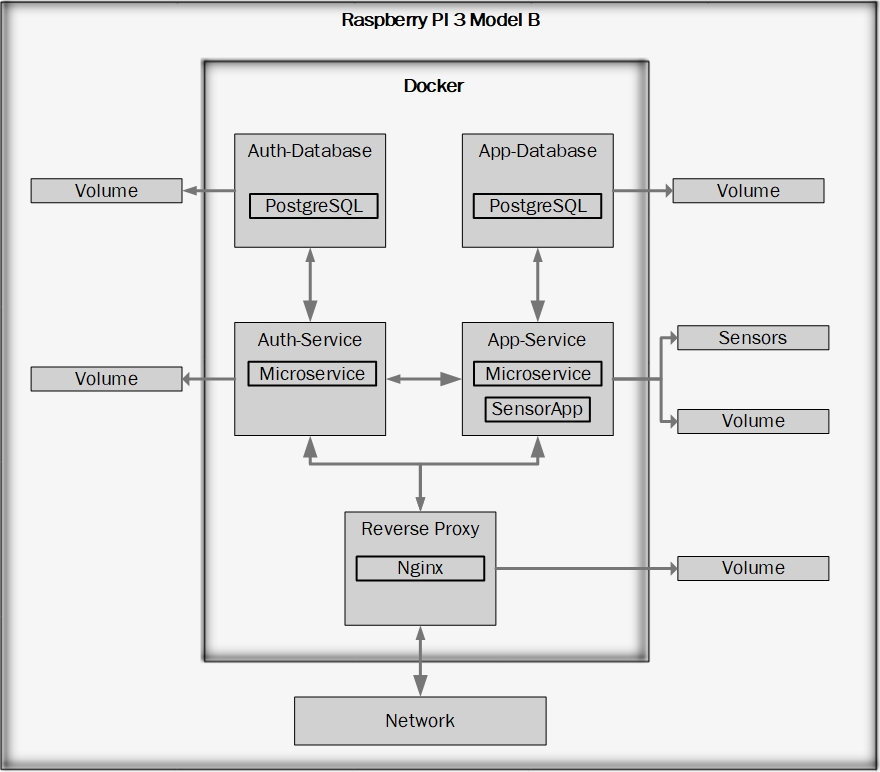
\includegraphics[scale=0.65]{\imageDir/pi-docker-infrastructure.jpg}
		\caption{\emph{Raspberry PI Docker} Infrastruktur}
		\label{fig:rapsi-docker-infrastructure}
	\end{figure}
\end{center}
Die Abbildung \ref{fig:rapsi-docker-infrastructure} zeigt die implementierte \emph{Docker} Infrastruktur, wie sie am \emph{Raspberry PI} gehostet wird. Da die Daten der \emph{Docker-Container} persistent gehalten werden müssen, werden die Daten in den \emph{Containern} in Verzeichnissen gehalten, die auf den \emph{Host} über ein \emph{Volume Mapping} gebunden sind. Der \emph{Docker Container App-Service} benötigt privilegierte Rechte, damit die Sensorapplikation mit der angeschlossenen \emph{Hardware} des \emph{Raspberry PI} kommunizieren kann. 
\newline
\newline
Der Quelltext \ref{src:test-docker-compose} zeigt den Inhalt der \emph{docker-compose.yml}, welche die \emph{Docker} Infrastruktur für \emph{RPISec} am \emph{Raspberry PI} definiert. Die in der Datei vorkommenden Textfragmente im Format \emph{\$\{...\}} stellen Variablen dar, die \emph{Docker-Compose} entweder aus einer Datei mit dem Namen \emph{.env}, die auf derselben Ebene wie die \emph{docker-compose.yml} platziert werden muss, oder aus den Umgebungsvariablen des Benutzers, mit dem die Infrastruktur erstellt wird, auflöst. Sollten Variablen nicht auflösbar sein, so wird eine entsprechende Meldung auf die Konsole ausgegeben.
\begin{code}
	\caption{docker-compose.yml für RPISec am \emph{Raspberry PI}}
	\yamlFile{\dockerRPIDir/docker-compose.yml}
	\label{src:test-docker-compose}
\end{code}
\ \newline
Das Bauen der Infrastruktur und Starten der Services dauert am \emph{Raspberry PI} relativ lange, da nur wenig Speicher zur Verfügung steht, es sich um eine ARM-Architektur handelt und das Speichermedium eine \emph{MicroSD} Karte ist. Ebenso ist die Performance der Services nicht herausragend, jedoch kann die Applikation auf dem \emph{Raspberry PI} problemlos ausgeführt werden.  